\subsubsection{\theoryC{High mass dilepton searches at HE-LHC ($ee, \mu\mu, \tau\tau$)}}
\label{subsubsec:hr_lep}
\contributors{C. Helsens, D. Jamin, M. Selvaggi}\rt{There are comments to address.}
%{\bf Authors: C. Helsens$^1$, D. Jamin$^2$, M. Selvaggi$^3$}\\
%\newline
%$^1$CERN EP-Departement, CH-1211 Geneva 23, Switzerland email: {\tt B.C. clement.helsens@cern.ch}\\
%$^2$Academia Sinica, Institute of  Physics, Taipei, Taiwan\\


%\newcommand*{\Zp}{\ensuremath{Z^{\prime}}}
%\newcommand*{\ZpSSM}{\ensuremath{Z^{\prime}_{\mathrm{SSM}}}}
%\newcommand*{\Z}{\ensuremath{Z}}
%\newcommand*{\Zptata}{\ensuremath{Z^{\prime}\rightarrow \tau\tau}}
%\newcommand*{\Zpee}{\ensuremath{Z^{\prime}\rightarrow e e}}
%\newcommand*{\Zpmumu}{\ensuremath{Z^{\prime}\rightarrow \mu\mu}}
%\newcommand*{\Zpll}{\ensuremath{Z^{\prime}\rightarrow \ell\ell}}
%\newcommand*{\Zptt}{\ensuremath{Z^{\prime}\rightarrow \ttbar}}
%\newcommand*{\ptZp}{\ensuremath{p_{\text{T}}^{\ensuremath{Z^{\prime}}}}}
%\newcommand*{\intlumihelhc}{\ensuremath{\mathcal{L}=15\text{ ab}^{-1}}}


%%%%%%%%%%%%%%%%%%%%%%%%%%%%%%%%%%%%%%%%%%%%%%%%%%%%%%%%%%%%%%%%%%%%%%%%%%%%%%%%%%%%%%%%%%%%
%\subsubsection{Introduction}
%\paragraph*{Introduction}
Models with extended gauge groups often feature additional U(1) symmetries with corresponding heavy spin-1 bosons. These bosons, generally referred to as $\Zp$, would manifest themselves as a narrow resonance in the dilepton invariant mass spectrum. Among these models are those inspired by Grand Unified Theories, motivated by gauge unification, or a restoration of the left-right symmetry violated by the weak interaction. Examples include the $\Zp$ bosons of the $E_{6}$ motivated theories~\cite{London:1986jz,Joglekar:2016yap,Langacker:2008yv} and Minimal models~\cite{Salvioni:2009mt}. The Sequential Standard Model (SSM)~\cite{Langacker:2008yv} posits a $\ZpSSM$ boson with couplings to fermions that are identical to those of the Standard Model $\Z$ boson.

The decay products of heavy resonances are in the multi-TeV regime and the capability to reconstruct their momentum imposes stringent requirement on the detector design. In particular, reconstructing the track curvature of multi-TeV muons requires excellent position resolution and a large lever arm. In this section, the expected sensitivity is presented for a \Zpll\ (where $\ell=\mathrm{e},\mu$) and \Zptata\ separately.

%%%%%%%%%%%%%%%%%%%%%%%%%%%%%%%%%%%%%%%%%%%%%%%%%%%%%%%%%%%%%%%%%%%%%%%%%%%%%%%%%%%%%%%%%%%%
%\subsubsection{Monte Carlo Samples}
%\paragraph*{Monte Carlo Samples}
Monte Carlo simulated event samples were used to simulate the response of the future detector to signal and backgrounds. The muon momentum resolution is assumed to be $\sigma(p)/p \approx 20\%$ at $\pt= 20 $TeV. Signals are generated with \pythia~8.230~\cite{Sjostrand:2014zea} using the leading order cross-section from the generator.
All lepton flavour decays of the $\ZpSSM$ are generated assuming universality of the couplings.
The Drell-Yan background has been generated using \MGvATNLO 2.5.2~\cite{Alwall:2014hca} at leading order only. A k-factor of 2 is applied to all the background processes. \rt{In every contribution you put a $k$-factor of 2 on the background. This seems an irrelevant arbitrary assumption.}

%%%%%%%%%%%%%%%%%%%%%%%%%%%%%%%%%%%%%%%%%%%%%%%%%%%%%%%%%%%%%%%%%%%%%%%%%%%%%%%%%%%%%%%%%%%%
%\subsubsection{Event Selection}
%\paragraph*{Event Selection}
Events are required to contain two leptons with $\pt > 0.5$~TeV, $|\eta|<4$. For ditau final state we focus on the most sensitive fully hadronic channel only. The ditau event selection requires two jets with $p_{T} > 0.5$>~TeV and $|\eta|<2.5$ identified as $\tau$'s. To ensure no overlap between the $\ell$ and $\tau$ final states, jets containing leptons with $\pt > 100$~GeV are vetoed. Finally, requirements of $\Delta \phi(\tau_1, \tau_2)> 2.4$ and $2.4<\Delta R(\tau_1, \tau_2)<4.6$ are applied.
Mass dependent cuts applied to maximise the signal to background ratio are summarised in \tabb{tab:leptonicresonances:selectiontautau}.

The left and central panels of \fig{fig:leptonicresonances:masses} show the invariant mass distribution for a 6~TeV signal in the $ee$ and $\mu\mu$ channels. The mass resolution is better for the $ee$ channel, as expected. The right panel of \fig{fig:leptonicresonances:masses} shows the transverse mass~\footnote{The transverse mass is defined as $m_{T}  =  \sqrt{2\ptZp*\met*(1-\cos\Delta\phi(\Zp,\met))}$.}
of a 6~TeV signal for the $\tau\tau$ channel.
Several proxies for the true resonance mass have been tested, such as the invariant mass of the two taus, with and without correction for the missing energy. The transverse mass provided the best sensitivity and was therefore used to set limits and determine the discovery reach.

\begin{table}[htbp]
   \centering
\begin{tabular}{l|l|c|r}
   $\Zp$ mass [TeV] &  $\Delta \phi(\tau_1, \tau_2)$&  $\Delta R(\tau_1, \tau_2)$ & $\met$\\
  \hline
   $2$ & > 2.4 & > 2.4 and < 3.9 & > 80 GeV\\
   $4$ & > 2.4 & > 2.7 and < 4.4 & > 80 GeV\\
   $6$ & > 2.4 & > 2.9 and < 4.4 & > 80 GeV\\
   $8$ & > 2.6 & > 2.9 and < 4.6 & > 80 GeV\\
  $10$ & > 2.8 & > 2.9 and < 4.1 & > 60 GeV\\
  $12$ & > 2.8 & > 3.0 and < 3.6 & > 60 GeV\\
  $14$ & > 3.0 & > 3.0 and < 3.3 & > 60 GeV\\
  \end{tabular}
  \caption{List of mass dependent cuts optimised to maximise the sensitivity for the \Zptata\ search.}
  \label{tab:leptonicresonances:selectiontautau}
\end{table}


\begin{figure}[htbp]
  \centering
  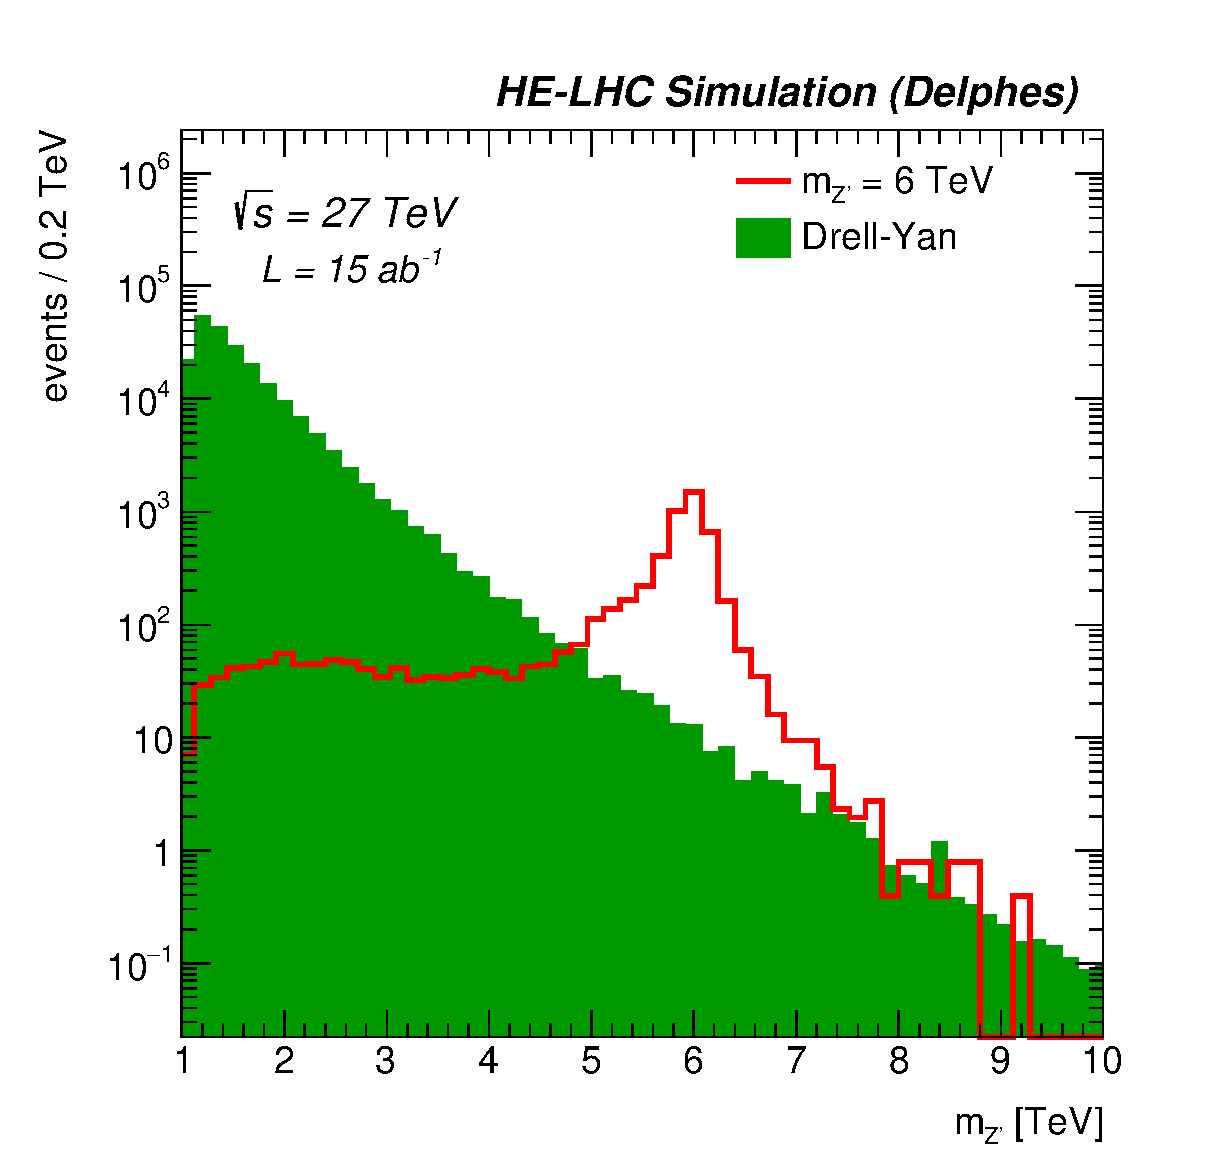
\includegraphics[width=0.32\columnwidth]{\main/section7OtherSignatures/img/Zpee_mzp_sel0_nostack_log.eps}
  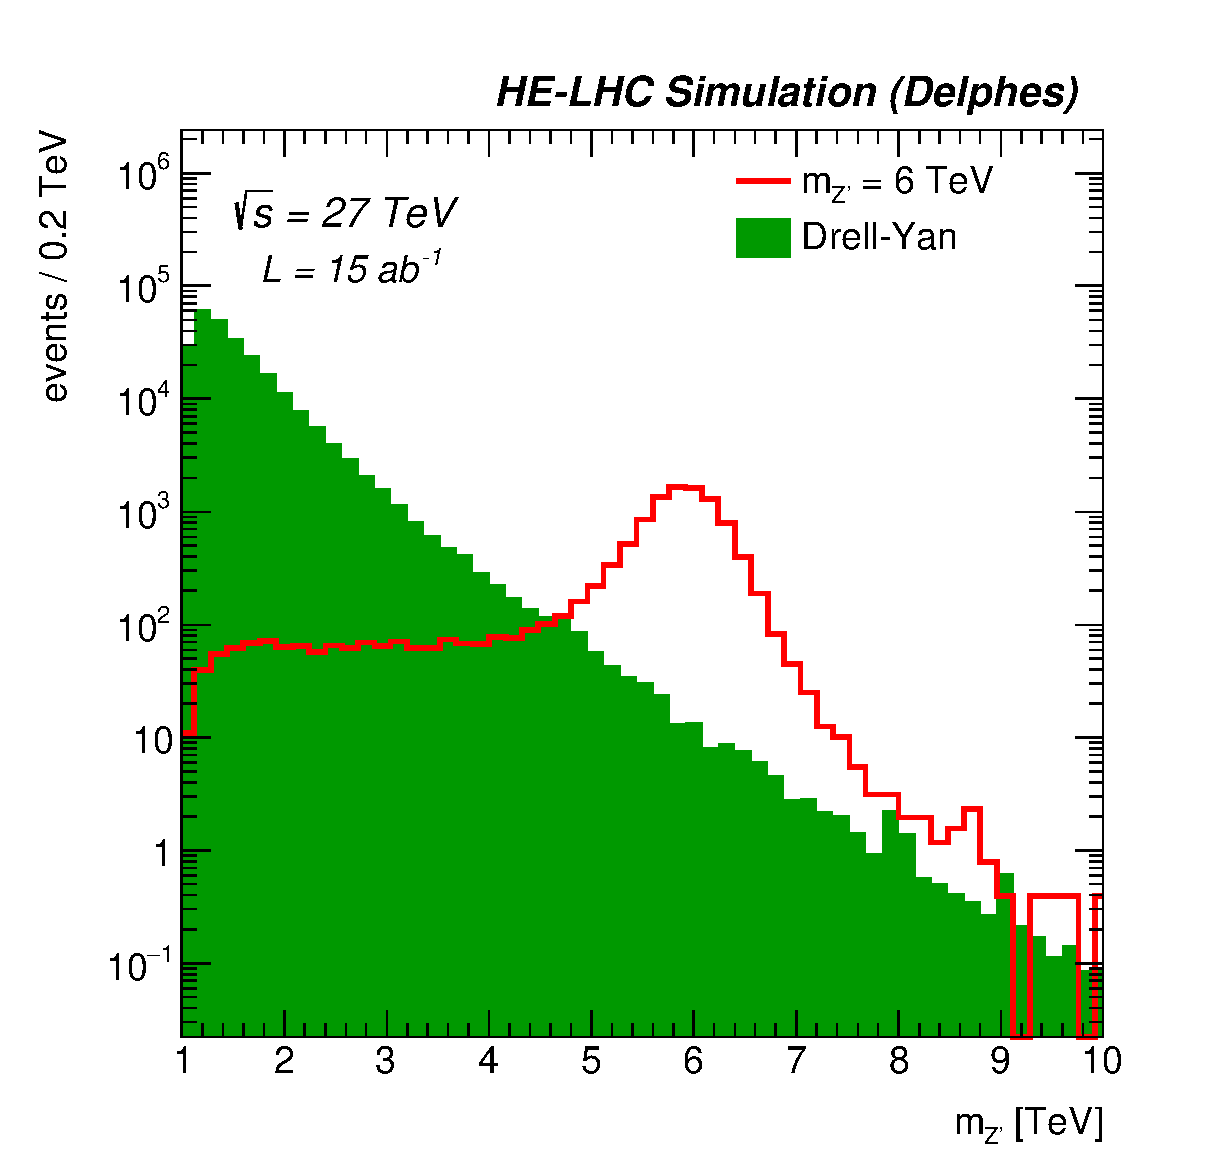
\includegraphics[width=0.32\columnwidth]{\main/section7OtherSignatures/img/Zpmumu_mzp_sel0_nostack_log.eps}
  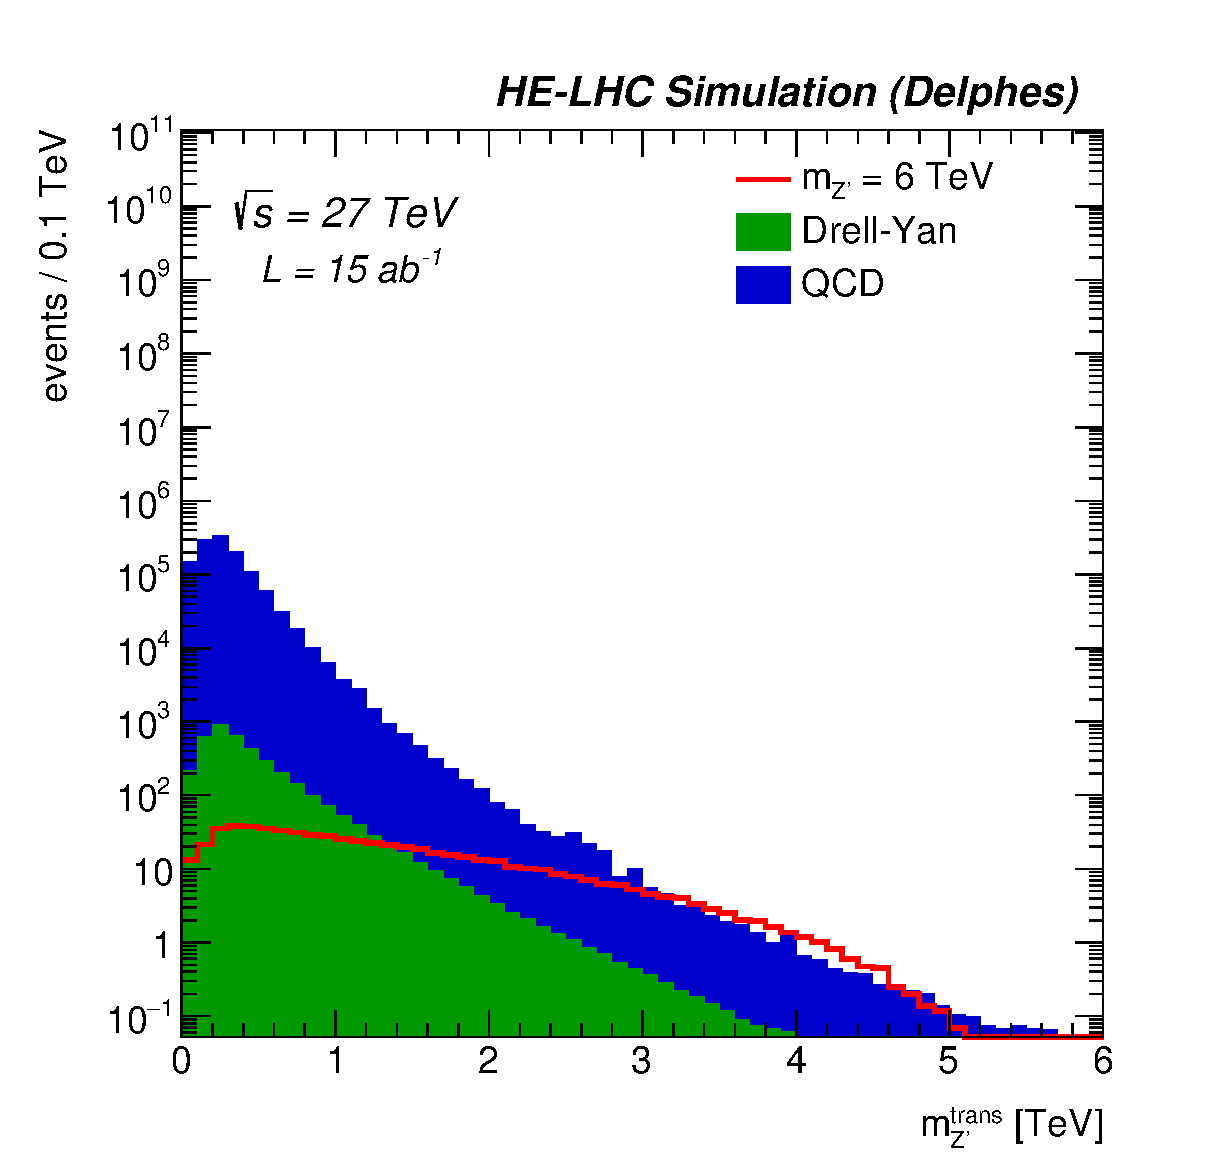
\includegraphics[width=0.32\columnwidth]{\main/section7OtherSignatures/img/Zptautau_mt_sel0_nostack_log.eps}
  \caption{Left, center: Invariant mass for a 6~TeV signal after full event selection for ee channel (left) and $\mu\mu$ channel (center). Right: Transverse mass for a 6~TeV signal after full event selection for the $\tau\tau$ channel. }
  \label{fig:leptonicresonances:masses}
\end{figure}
%\MS{need editing / style}

%%%%%%%%%%%%%%%%%%%%%%%%%%%%%%%%%%%%%%%%%%%%%%%%%%%%%%%%%%%%%%%%%%%%%%%%%%%%%%%%%%%%%%%%%%%%
%\subsubsection{Results and discussion}
%\paragraph*{Results and discussion}
Hypothesis testing is performed using a modified frequentist method based on a profile likelihood that takes into account the systematic uncertainties as nuisance parameters that are fitted to the expected MC. For the $ee$ and $\mu\mu$ analyses, the dilepton invariant mass is used as the discriminant, while for the $\tau\tau$ channel the transverse mass is used. A 50\% uncertainty on the background normalisation is assumed.

The exclusion limit obtained using \intlumihelhc\ of data for the combination of the ee and $\mu\mu$ channels is shown in \fig{fig:leptonicresonances:resultsll} (left). Figure~\ref{fig:leptonicresonances:resultsll} (right) shows the integrated luminosity required to reach a $5\sigma$ discovery for the leptonic resonances as a function of the mass of the heavy resonance. The \Zpee\ and \Zpmumu\ channel display very similar performances, due to the low background rates. We conclude therefore that the reference detector design features near to optimal performances for searches involving high \pT\ muon final states. Figure~\ref{fig:leptonicresonances:resultstautau} shows the exclusion limits for 15 ab$^{-1}$ of data (left) and the required integrated luminosity
versus mass to reach a $5\sigma$ discovery (right) for the ditau resonances. \rt{Comment on this being weaker than $ee$ and $\mu\mu$}.

%The discovery potential for high mass resonances decaying to $ee$, $\mu\mu$ and $\tau\tau$ has been studied using as a benchmark the \ZpSSM\ model.
In summary, the large centre of mass energy of the HE-LHC obviously translates in a correspondingly large mass reach. In the benchmark \ZpSSM mode, in the $ee$ and $\mu\mu$ final states, masses up to 12~TeV can be excluded or discovered. Heavy resonance decaying to $\tau$ leptons reconstructed in the hadronic decay mode are more challenging, but we would be able to probe masses up to 6~TeV.

  \begin{figure}[htbp]
  \centering
  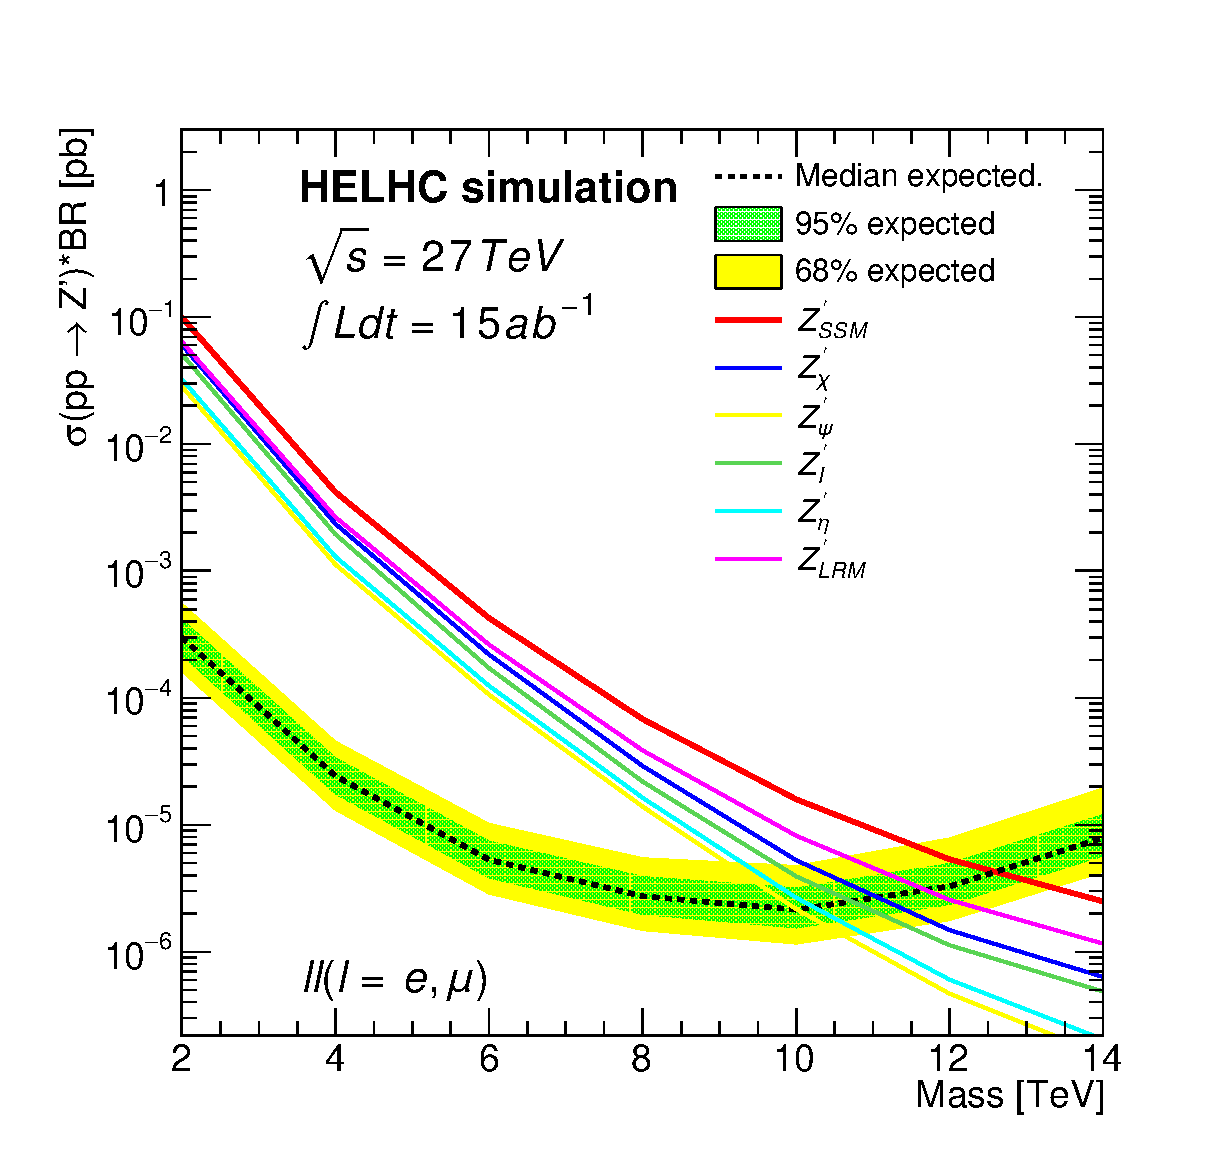
\includegraphics[width=0.45\columnwidth]{\main/section7OtherSignatures/img/lim_Zprime_ll_helhc_v01_allxs.eps}
  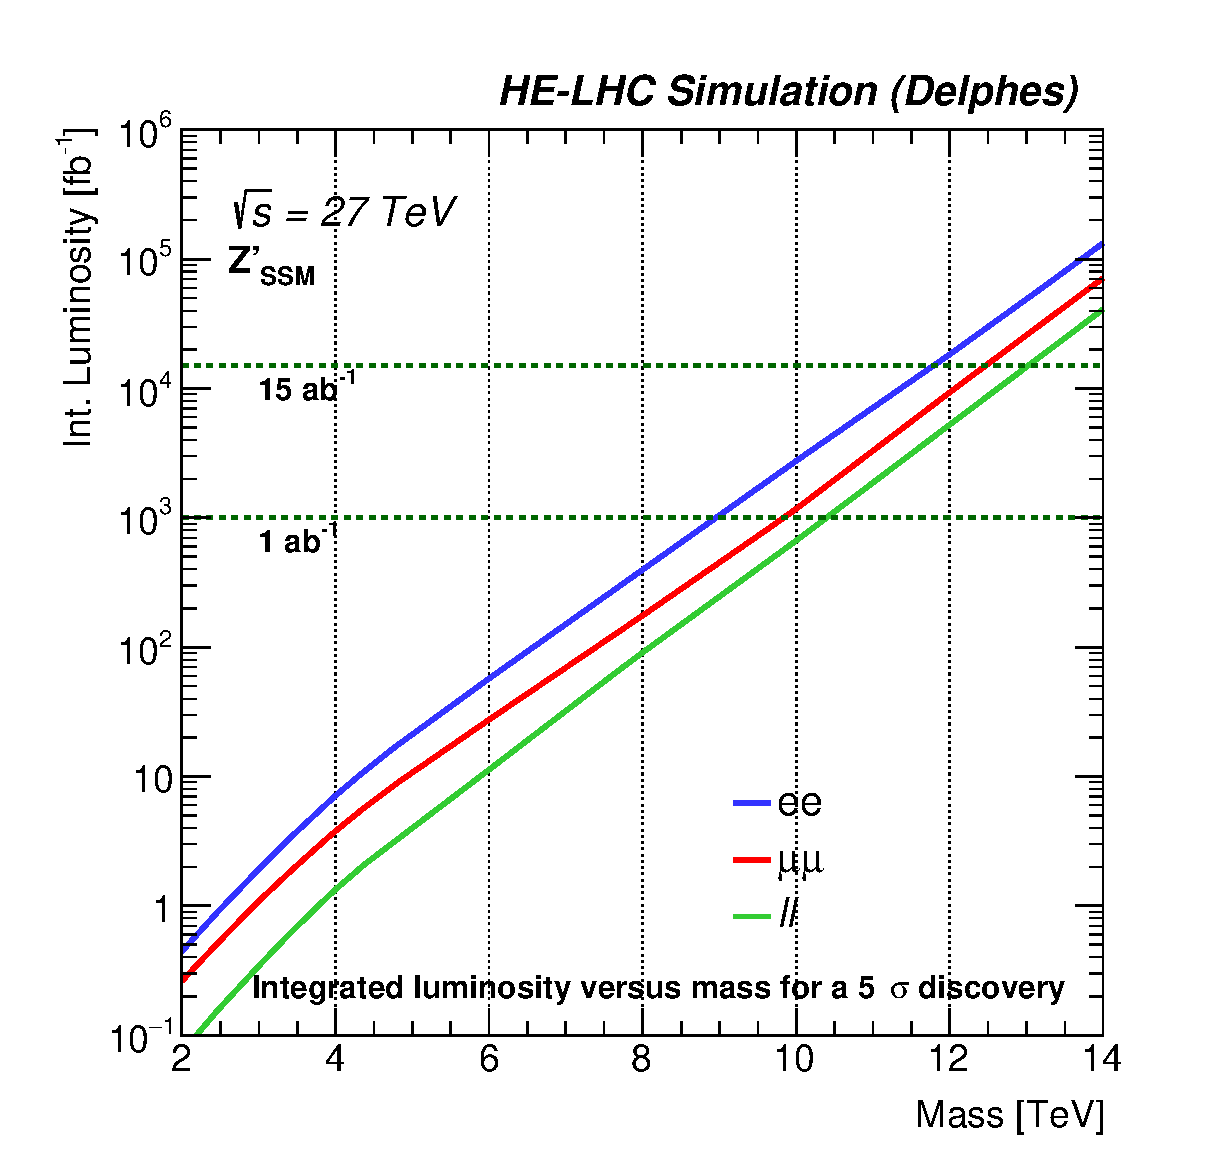
\includegraphics[width=0.45\columnwidth]{\main/section7OtherSignatures/img/DiscoveryPotential_ll_comb_rootStyle.eps}
  \caption{Limit versus mass for the dilepton (ee,$\mu\mu$) channel (left) and luminosity for a $5\sigma$ discovery (right) comparing ee,$\mu\mu$ and combined channels. }
  \label{fig:leptonicresonances:resultsll}
\end{figure}

\begin{figure}[htbp]
  \centering
    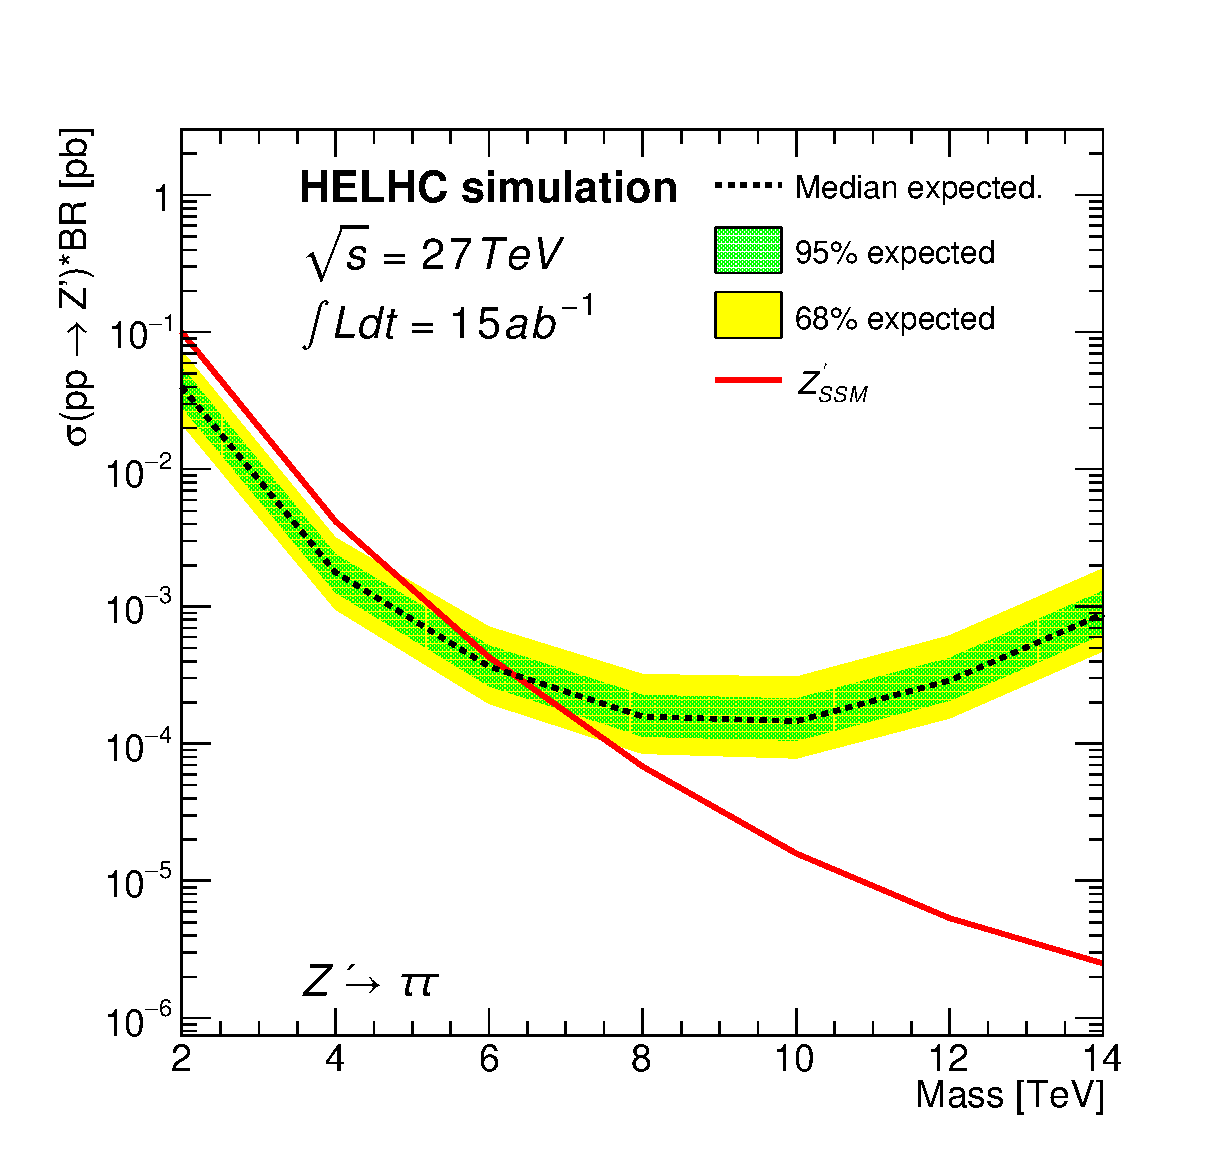
\includegraphics[width=0.45\columnwidth]{\main/section7OtherSignatures/img/lim_Zprime_tautau_helhc_v01.eps}
    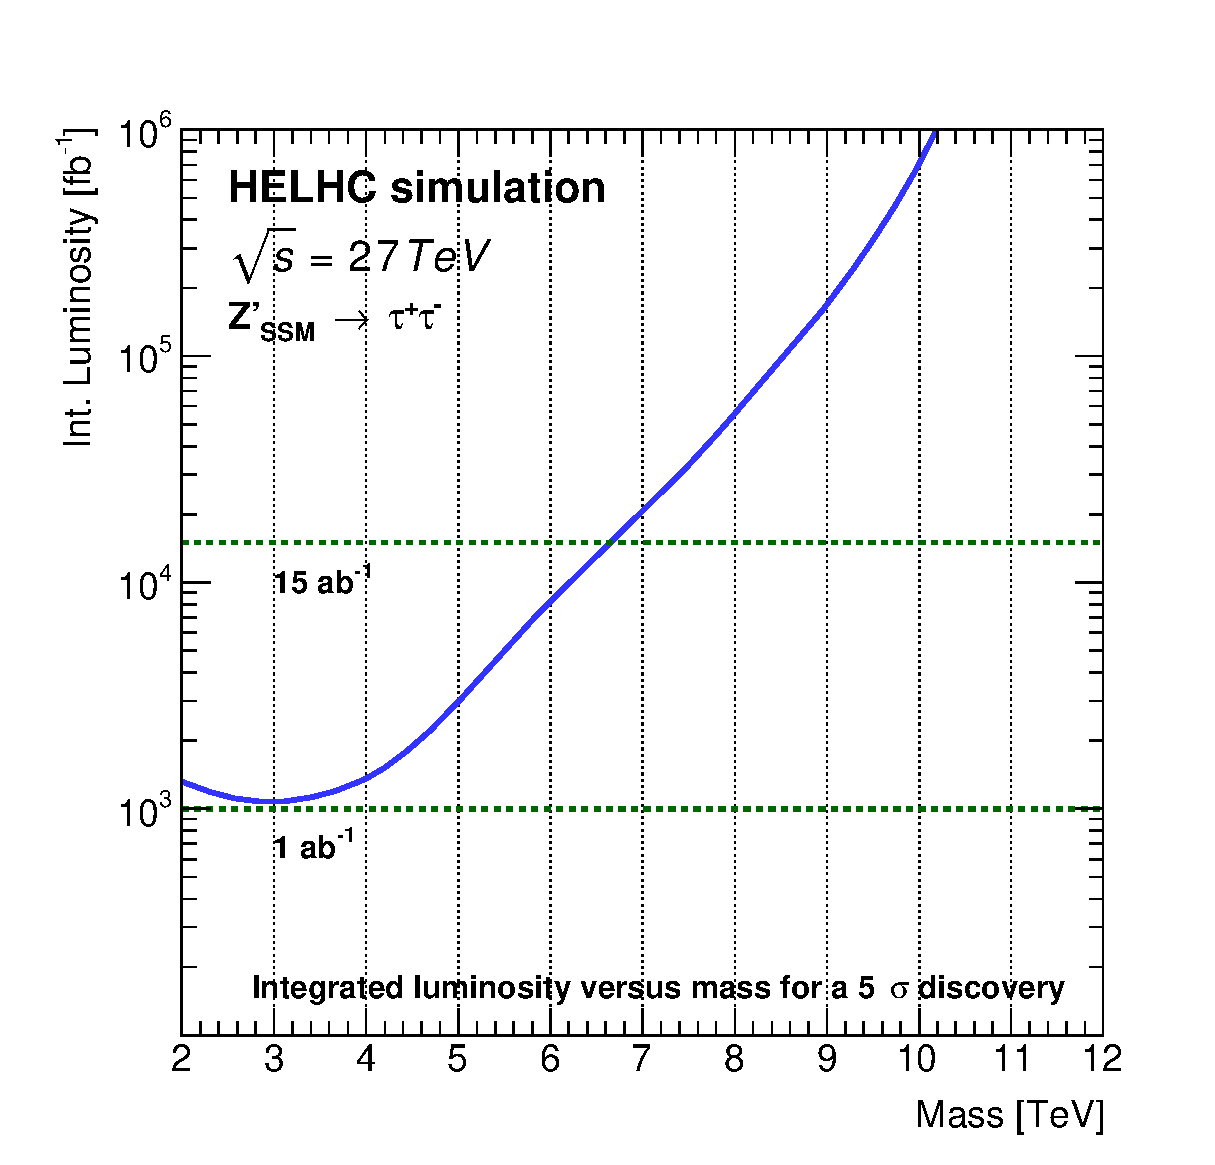
\includegraphics[width=0.45\columnwidth]{\main/section7OtherSignatures/img/DiscoveryPotential_tautau_rootStyle.eps}
  \caption{Limit versus mass for the ditau channel (left) and luminosity for a $5\sigma$ discovery (right). }
  \label{fig:leptonicresonances:resultstautau}
\end{figure}
